\documentclass[fleqn]{VUMIFKompMagistrinis}
\usepackage{algorithmicx}
\usepackage{algorithm}
\usepackage{algpseudocode}
\usepackage{amsfonts}
\usepackage{amsmath}
\usepackage{bm}
\usepackage{caption}
\usepackage{color}
\usepackage{float}
\usepackage{graphicx}
\usepackage{listings}
\usepackage{subfig}
\usepackage{wrapfig}

% Titulinio aprašas (nereikalingus elementus užkomentuoti)
\university{Vilniaus universitetas}
\faculty{Matematikos ir informatikos fakultetas}
\institute{Informatikos institutas}  % Užkomentavus šią eilutę - institutas neįtraukiamas į titulinį
\department{Programų sistemų BAKALAURO STUDIJŲ PROGRAMA}
\papertype{Kursinis darbas}
\title{Ligų aptikimas naudojant plaučių echoskopiją}
\titleineng{Detecting diseases with lung ultrasound}
\author{Justas Baniulis}
\status{4 kurso, 1 grupės studentas}
% \secondauthor{Vardonis Pavardonis}   % Pridėti antrą autorių
% \thirdauthor{Vardonis Pavardonis}   % Pridėti antrą autorių
% \fourthauthor{Vardonis Pavardonis}   % Pridėti antrą autorių
\supervisor{asist. dr. Tomas Plankis}
% \reviewer{doc. dr. Vardauskas Pavardauskas}
\date{Vilnius \\ \the\year}

% Nustatymai
% \setmainfont{Palemonas}  % Pakeisti teksto šriftą į Palemonas (turi būti įdiegtas sistemoje)
\bibliography{bibliografija}  % Literatūros šaltinių aprašų failas bus bibliografija.bib

\begin{document}
\maketitle

\tableofcontents

% \santrauka{Santrauka}
% Glaustai aprašomas darbo turinys: pristatomi darbo tikslai, analizuotos ir
% tirtos problemos, atlikti eksperimentai bei padarytos išvados, gautos
% rekomentacijos. Santraukos apimtis ne didesnė nei 0,5 puslapio. Santraukų gale
% nurodomi darbo raktiniai žodžiai. 
% Nurodomi iki 5 svarbiausių temos raktinių žodžių (terminų).
% Vienas terminas gali susidėti iš kelių žodžių.
% \raktiniaizodziai{raktinis žodis 1, raktinis žodis 2, raktinis žodis 3, raktinis žodis 4, raktinis žodis 5}

%\summary{Summary}
%Santrauka anglų kalba. Santraukos apimtis ne didesnė nei 0,5 puslapio.
% \keywords{keyword 1, keyword 2, keyword 3, keyword 4, keyword 5}


\sectionnonum{Įvadas}
% Įvade aprašomi darbo tikslai, 
Daug žmonių kenčia nuo plaučių ligų, turime didelį mirtingumą, todėl reikia pagerinti diagnozės procesą. Echoskopija daryti yra pigu, bet reikia patyrusių specialistų ir laiko interpretuoti gaunamą vaizdą. Darbą palengvintų ištreniruoti neuroniniai tinklai. Šio darbo tikslas yra analizuoti ir palyginti giliojo mokymosi modelius, kurie, naudojantis echoskopinėmis nuotraukomis, aptinka dvi dažniausias plaučių ligas žmonių populiacijoje - COVID-19 ir pneumoniją (plaučių uždegimą) . 
% nurodomas temos aktualumas, motyvacija,
% formuluojamas sprendžiamas uždavinys ir siekiami rezultatai.

% Aptariamos teorinės darbo prielaidos bei metodika, apibrėžiamas tiriamasis
% objektas, apibūdinami su tema susiję literatūros ar kitokie šaltiniai, temos
% analizės tvarka, darbo atlikimo aplinkybės


\section{Transformerių neuroninis tinklas}
\subsection{Įžanga}
2021 metų rugsėjį elektrotechnikos ir elektronikos inžinierių instituto (angl. IEEE) konferencijos „IEEE International Conference on Image Processing“ publikuotame straipsnyje „POCFormer: A Lightweight Transformer Architecture for Detection of COVID-19 Using Point of Care Ultrasound“ autoriai sukūrė neuroninio tinklo architektūrą, kuri geba klasifikuoti plaučių echoskopijos nuotraukas\cite{PAY21}. Pasak straipsnio autorių, COVID-19 diagnozė naudojantis patvirtintomis priemonėmis, kaip PGR tyrimai, nors ir yra labai tiksli, tačiau užtrunka labai daug laiko ir dėl to negali būti naudojamos dideliu mastu. Pagal straipsnio autorius, technologiškai patobulinti mobilūs echoskopijos įrenginiai leidžia greičiau ir patogiau išgauti echoskopinę nuotrauką ir jie yra vis dažniau naudojami tarp sveikatos priežiūros specialistų. Straipsnio autoriai teigia, kad šių mobilių echoskopijos įrenginių trūkumas yra tai, kad gautus echoskopijos rezultatus gali analizuoti ir ligą diagnozuoti tik labai patyręs specialistas, o įgauti patirtį užtrunka laiko ir yra sunku. Straipsnio autoriai, kad palengvintų sveikatos priežiūros specialistų darbą interpretuojant gautas nuotraukas, automatizavo COVID-19 ir bakterinio plaučių uždegimo nustatymą iš echoskopinės nuotraukos. Apžvelgsime straipsnio autorių sukūrtą klasifikacijos modelį „POCFormer“, paremtą transformerių neuroninio tinklo architektūra, ir klasifikuojantį nuotrauką į COVID-19, bakterinio plaučių uždegimo, sveikų plaučių klases. \cite{PAY21}

% Straipsnio autoriai sukurė modelį, kuris diagnozuoja COVID-19 ir bakterinį plaučių uždegimą, prilygsta tikslumu profesionalius sveikatos priežiūros specialistus ir yra prieinamas masiniam naudojimui, dėl greitos diagnozės.

\subsection{Architektūra}

\subsubsection{Bendras aprašymas}
Autorių sukurtą modelį sudaro dvi pagrindinės dalys: 
\begin{enumerate}
    \item Regos tranformerių neuroninis tinklas (angl. „Vision transformer“, sutrumpinimas „ViT“), kuris išekstrahuoja požymius iš suskaidytos echoskopinės nuotraukos derinant tos nuotraukos dalis su pozicijos įterpiniais \cite{PAY21}. Ši dalis aprašoma plačiau \ref{sec:vit} skyriuje.
    \item Tiesinis tranformerių neuroninis tinklas (angl. „linear transformer“, sutrumpinimas „Linformer“), kuris atlieka požymių, gautų iš „Vision transformer“ enkodinimą \cite{PAY21}. Ši dalis aprašoma plačiau \ref{sec:linformer} skyriuje.
\end{enumerate}
\par
Modelis taip pat turi du mažesnius sluoksnius:
\begin{enumerate}
    \item Prieš paduodant tranformerių neuroniniui tinklui nuotrauką, pirmame sluoksnyje ji yra suskaidoma į atskiras dalis. Tuomet dalys ištiesinamos, sukuriama dalių linijinė projekcija ir gauti vektoriai perduodami transformerių blokams. \cite{PAY21}
    \item Architektūroje egzistuoja paskutinysis „tankusis“ (arba pilnai sujungtų sąryšių) sluoksnis, kuris priima „Vision transformer“ ir „Linformer“ transformerių tinklų požymius ir paverčia juos klasių (COVID-19, bakterinis plaučių uždegimo, sveikų plaučių) išeitimi. \cite{PAY21}
\end{enumerate}
Aukšto lygio „POCFormer" modelio architektūra iliustruota \ref{img:POCFormer} paveikslėlyje .
\begin{figure}[H]
    \centering
    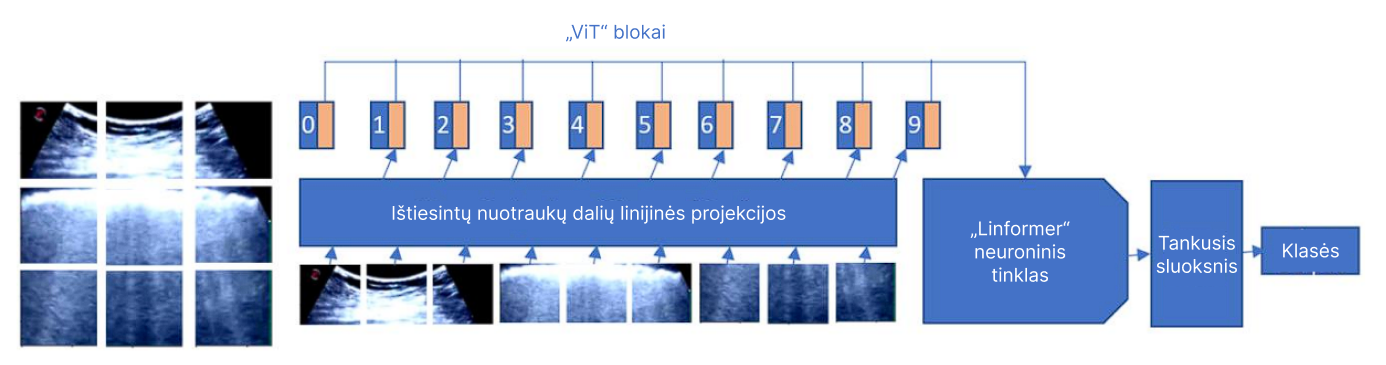
\includegraphics[scale=0.45]{img/transformerisMain.png}
    \caption{Aukšto lygio „POCFormer" modelio architektūra \cite{PAY21}}
    \label{img:POCFormer}
\end{figure}

\subsubsection{„ViT“ dalis}
\label{sec:vit}
\par
Pirmasis transformerių neuroninis tinklas buvo pristatytas 2017 metais „Attention is All You Need“ straipsnyje. Šio straipsnio autorių sukurta neuroninio tinklo architektūra skirta skaitmeniniam natūraliosios kalbos apdorojimui - dėmesio sutelkimo mechanizmas leidžia modeliui suprasti sąryšius tarp skirtingų tekstinių duomenų dalių ir suprasti kontekstą bei sąryšius jose. \cite{tranformeris}
\par
„Vision transformer“ modelis buvo pristatyas 2021 metų straipsnyje „An Image is Worth 16x16 Words: Transformers for Image Recognition at Scale“. Pasak šio straipsnio autorių, transformerių neuroninis tinklas gali būti naudojamas ne tik skaitmeniniam natūraliosios kalbos apdorojimui, bet ir nuotraukų klasifikacijos uždaviniams \cite{dosovitskiy2021image}. „Vision transformer“ modelis nuotrauką suskaido į atskiras dalis ir jos linijine projekcija sudedamos į vektorių kartu su pozicijos įterpiniu, kad modelis žinotų dalių originalią poziciją. Modelio pagrindinė dalis yra enkodinimo blokas, kurį sudaro keli dėmesio sutelkimo sluoksniai ir daugiasluoksnio perceptrono blokai. Dėmesio sutelkimo mechanizmas, kaip ir skaitmeniniame natūraliosios kalbos modelyje, leidžia modeliui įvertinti atskirų nuotraukų dalių globalius kontekstinius ryšius bei lokalųjį kontekstą. Taip pat prieš daugiasluoksnio perceptrono blokus yra du sluoksniai su gausinio tiesinio vieneto (angl. sutrumpinimas „GELU“) aktyvacijos funkcija, kuri leidžia tinklui mokintis sudėtingus šablonus (žr. formulę \ref{eq:gelu}) ir sluoksnio normalizacija (angl. sutrumpinimas „LayerNorm“) (žr. formulę \ref{eq:layernorm}), kuri stabilizuoja neuroninį tinklą normalizuojant kiekvieno sluoksnio požymių įvestis. Blokus seka praleidimo jungtys, kurios padeda išspręsti nykstančio gradiento problemą. \cite{dosovitskiy2021image}
\begin{equation}
    \centering\label{eq:gelu}
    \text{GELU}(x) = x \Phi(x)
\end{equation}
\par
\(\Phi(x)\) - normalaus atsitiktinio dydžio pasiskirstymo funkcija. 
\begin{equation}\label{eq:layernorm}
    \centering
    \text{LayerNorm}(x) = \gamma \odot \frac{x - \mu}{\sqrt{\sigma^2 + \epsilon}} + \beta
\end{equation}
\par
\( x \) - įvesties vektorius, t.y sluoksnio išvestis prieš normalizaciją.
\( \mu \) ir \( \sigma^2 \) - vidurkis ir variacija, apskaičiuojami kiekvieno duomenų taško požymių ašyse.
\( \epsilon \) - maža konstanta skaitmeniniam stabilumui užtikrinti, užkerta kelią dalybai iš nulio, kai variacija yra labai maža.
 \( \gamma \) ir \( \beta \) - mokomi „LayerNorm“ parametrai mastelio ir poslinkio keitimui. Rreguliuojami mokymo proceso metu.
\( \odot \) - elementų pagal elementus dauginimas.

\par
Transformerių neuroninių tinklų architektūra geba, pagal kūrėjus, per mažesnį epochų skaičių ir su mažiau duomenų gali pasiekti ir kai kuriuose uždaviniuose pralenkti konvoliucinių neuroninų tinklų (angl. CNN) architektūrų, kurios dažniausiai naudojamos nuotraukų klasifikacijai, metrikas \cite{dosovitskiy2021image}. Kadangi plaučių echoskopinių nuotraukų straipsnio rašymu metu buvo trūkumas, ši architektūra padėjo išspręsti mažo duomenų kiekio problemą. \cite{PAY21}   
\subsubsection{„Linformer“ dalis}
\label{sec:linformer}
Nors transformerių neuroninių tinklai prilygsta ar yra geresni CNN metrikų atžvilgiu, šių tinklų treniravimas ir naudojimas užima daug resursų dėl „Vision transformer“ dėmesio sutelkimo enkoderio sudėtingumo. Didelis parametrų skaičius apsunkina mobilių echoskopijos prietaisų darbą, nes jų atmintis ir skaičiavimo pajėgumai yra stipriai apriboti \cite{PAY21}. Dėl šios priežasties kūrėjai pasinaudojo „Linformer“ enkoderiu, 2020 metais pristatytu „Linformer: Self-Attention with Linear Complexity“ straipsnyje, kuris optimizavo tranformerių dėmesio sutelkimo mechanizmą. \cite{PAY21, wang2020linformer}.
\par
Pasak „Linformer“ enkoderio autorių, jų dėmesį sutelkančio mechanizmo sudėtingumas yra \( O(n) \), o originalaus „Vision transformer“ sudėtingumas yra \( O(n^2) \) laiko ir atminties atžvilgiu \cite{wang2020linformer}. Straipsnio autoriai sugebėjo optimizuoti enkodinimą aproksimuojant dėmesio sutelkimo mechanizmą su žemo rango matricos faktorizacija, parametrų dalinimusi tarp komponentų ir pridedant dvi linijines projekcijas apskaičiuojant reikšmes \cite{wang2020linformer}. Vieno komponento architektūra iliustruota paveiklėlyje \ref{img:linformer}.

\begin{figure}[H]
    \centering
    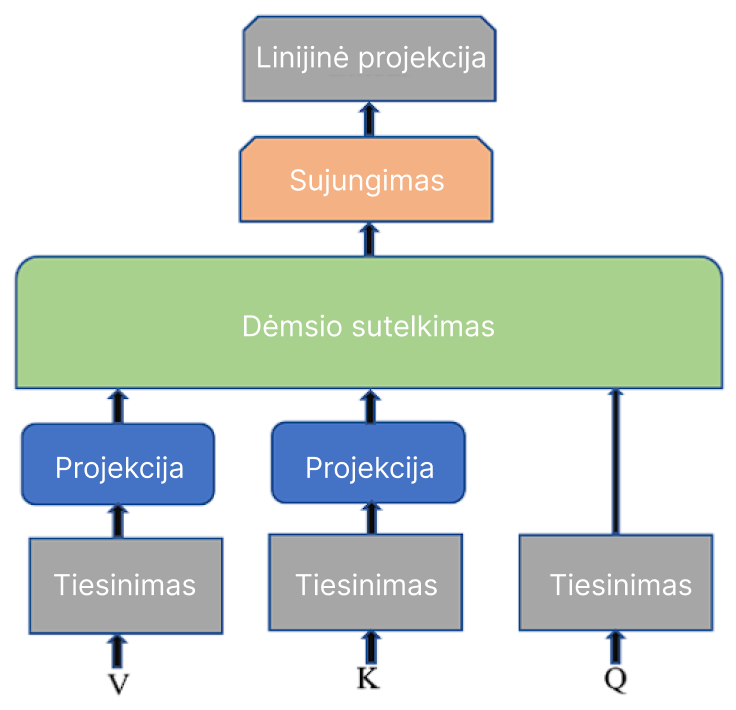
\includegraphics[scale=0.40]{img/linformer.PNG}
    \caption{Vieno „Linformer" komponento architektūra \cite{PAY21}}
    \label{img:linformer}
\end{figure}

\par
Pagal „POCFormer" modelio autorius, jų modelis, naudojantis „Linformer“ metodą, turi ženkliai mažesnį parametrų kiekį palyginus su kitais nuotraukų klasifikacijos ir skaitmeninio kalbos apdorojimo modeliais, paremtais transformerių neuroniniais tinklais (žr. lentelę \ref{tab:parametrai1}), o tai labai svarbu mobiliems echoskopijos prietaisams su ribotais resursais ir siekiant sveikatos priežiūros specialistams greitai nustatyti ligą. Be to, šis sprendimas, pasak autorių, leidžia naudotis tranformerių neuroninių tinklų mokymosi su lokaliais ir globaliais kontekstiniais ryšiais savybe, kuri svarbi išlaikant aukštas metrikas nuotraukų klasifikacijoje ir nustatant ligą. \cite{PAY21}

\begin{table}[H]\footnotesize
  \centering
  \caption{Transformerių neuroninių tinklų palyginimas \cite{PAY21, dosovitskiy2021image}}
  \begin{tabular}{|l|c|c|} \hline
    Modelis    & Parametrų kiekis \\
    \hline
    „BERT“ & \( 345 \cdot 10^6 \) \\
    „Vision transformer“ & \( \approx61 \cdot 10^6 \) \\
    \textbf{„POCFormer" daugelio klasių}  & \( \textbf{6.9} \cdot \textbf{10} ^ \textbf{6} \) \\
    \hline
  \end{tabular}
  \label{tab:parametrai1}
\end{table}

\subsection{Duomenys}
Autoriai teigia, jog modelio treniravimui naudojo atviros prieigos duomenų rinkinį, kuriame saugomi medicinos ekspertų sužymėti plaučių echoskopijos vaizdo įrašai ir nuotraukos iš pacientų\cite{PAY21}. Pasak autorių, treniravimo ir testavimo duomenų rinkiniai buvo sukurti naudojantis plaučių echoskopijos vaizdo įrašų kadrais ir nuotraukomis, kurie suskirstyti į tris kategorijas - COVID-19, bakterinio plaučių uždegimo ir sveikų plaučių. Pagal autorius, kad treniravimo, validacijos ir testavimo duomenų rinkinių klasės būtų subalansuotos, modelio nuostolių funkcijoje buvo panaudotas parametrų balansavimo mechanizmas (žr. formulę \ref{eq:weight_vector}), kuris parametrų vektoriuose klasėms, kurios turi mažiau duomenų, suteikia aukštesnį parametro reikšmę.\cite{PAY21}
\begin{equation}\label{eq:weight_vector}
    \text{weight\_vector} = \frac{1}{X/\min(X)}
\end{equation}
\( X \) - kiekvienos klasės nuotraukų kiekis
\par
Pagal autorius, dažniausiai pasitaikantys echoskopinių vaizdo įrašų kadrų ir nuotraukų požymiai yra A ir B linijos. Išgautiems kadrams, prieš pradedant treniravimą, autoriai pritaikė šias transformacijas, kad nuotraukos gautos iš skirtingų šaltinių būtų standartizuotos \cite{PAY21}:
\begin{enumerate}
    \item konvertuojamos nuotraukos į 224 \(\cdot\) 224 dimensiją.
    \item 8 bitų nuotraukoms atliekama normalizacija tarp reikšmių \([0,1]\) 
    \item nuotraukų vidurkis ir standartinis nuokrypis perskaičiuojami (žr. formules \ref{eq:transformerio}) 
\end{enumerate}
\begin{equation}\label{eq:transformerio}
\mu = \left( \frac{1}{n} \sum_{i=1}^{n} x_i \right), \quad
\sigma = \sqrt{\frac{1}{N} \sum_{i=1}^{N} (x_i - \mu)^2}
\end{equation}
\( x_i = [R_i, G_i, B_i]^T \) - raudonos, geltonos, mėlynos spalvos kanalai, \(\mu\) - nuotraukos vidurkis, \(\sigma\) - nuotraukos standartinis nuokrypis. 
\par
Straipsnio autoriai iš duomenų rinkinio priskyrė \(\approx400\) nuotraukų kiekvienai klasei. Toks, pagal autorių nuomone, mažas kiekis buvo pasirinktas norint pademonstruoti architektūros gebėjimą pasiekti aukštas metrikas naudojantis mažesniu duomenų rinkiniu, kadangi surinkti didelius duomenų kiekius medicinos srityje yra sunku, nes rinkimas reikalauja daug pastangų.\cite{PAY21}
\subsection{Apmokymas}
Straipsnio autoriai treniravo keturis klasifikacijos modelius - tris dviejų klasių klasifikavimo ir vieną daugelio klasių klasifikavimo \cite{PAY21}. Straipsnio autorių dvejų klasių modeliai susidaro iš:
\begin{enumerate}
    \item COVID-19 ir sveikų plaučių klasifikacija,
    \item COVID-19 ir bakterinio plaučių uždegimo klasifikacija,
    \item Bakterinio plaučių uždegimo ir COVID-19 klasifikacija
\end{enumerate}
\par 
Autoriai teigia jog, vykstant treniravimo procesui jie ieškojo geriausių hiperparametrų, kadangi „Vision transformer“ tinklas ir „Linformer“ modelis turi efektyviai veikti kartu \cite{PAY21}. Taip pat autoriai teigia, jog dviejų klasių modelių kūrimas ir sėkmingas treniravimas jiems padėjo parinkti hiperparametrų reikšmes ir daugelio klasių modeliui. Autorių pateikti naudojami hiperparametrai modeliuose pateikti \ref{tab:parametrai1} lentelėje. Mokymo epochų kiekio autoriai nepateikia. 
\begin{table}[H]\footnotesize
  \centering
  \caption{„POCFormer“ hiperparametrai \cite{PAY21}}
  \begin{tabular}{|l|c|c|} \hline
     & Daugelio klasių & Dvejų klasių \\
    \hline
    Sluoksnių kiekis &  32&  12 \\
    Paslėptų sluoksnių dydis &  64&  32 \\
    Daugiasluoksnio perceptrono dydis &  128&  128 \\
    Nuotraukos dalies dydis &  32&  32 \\
    Dėmesio sutelkimo „galvutės“ &  8&  8 \\
    Parametrų kiekis &  6,9 mln.&  2,8 mln. \\
    \hline
  \end{tabular}
  \label{tab:parametrai1}
\end{table}
\par
Autoriai treniravimui, validacijai ir testavimui naudojo PyTorch karkasą ir nuosavus kompiuterinius resursus, kuriuos sudarė Intel Core i7-9700K 4.7GHz procesorius ir RTX 2080 vaizdo plokštė su 8GB RAM. „POCFormer“ modelio kaštų funkcija yra kryžminės entropijos funkcija (žr. formulę \ref{eq:cross}) \cite{PAY21}.\begin{equation}\label{eq:cross}
\text{Cross Entropy Loss} = - \sum_{c=1}^{M} y_{o,c} \log(p_{o,c})
\end{equation}
\( p \) - prognozuojama tikimybė, jog stebimasis \(o\) priklauso \(c\)  klasei, o \(y\) yra dvejetainis rodiklis (0 arba 1), nusakantis ar klasė \(c\) yra teisingai klasifikuojama stebimam \(o\) \cite{PAY21}.
\subsection{Rezultatai}
Straipsnio autoriai ištreniruotų dvejų klasių modelių efektyvumui vertinti naudojo preciziškumo, tikslumo, F1, jautrumo ir specifiškumo  metrikas (žr. \ref{tab:statistikos1} lentelę) ir daugelio klasių modelio efektyvumui vertinti naudojo atkūrimo, preciziškumo, F1, specifiškumo ir jautrumo metrikas (žr.\ref{tab:statistikos2} lentelę ). 
\par
Straipsnio autorių modeliai efektyviai klasifikuoja COVID-19, bakterinio uždegimo ir sveikų plaučių klases - visų metrikų reikšmės yra aukštos. Aukštos preciziškumo ir tikslumo reikšmės rodo, jog modelis pateikia mažai klaidingai teigiamų ir klaidingai neigiamų spėjimų. Visuose modeliuose aukštas F1 rodo, jog architektūra yra gerai subalansuota.
\begin{table}[H]\footnotesize
  \centering
  \caption{„POCFormer“ dvejų klasių modelių metrikos \cite{PAY21}}
  \begin{tabular}{|l|c|c|c|c|c|} \hline
    Modelis & Preciziškumas. & Tikslumas & F1 & Jautrumas & Specifiškumas \\
    \hline
    COVID-19 ir sveiki plaučiai & 0.87 & 0.91 & 0.92 & 0.83 & 0.97 \\
    COVID-19 ir bakterinis uždegimas & 0.93 & 0.95 & 0.93 & 1.00 & 0.88 \\
    Bakterinis uždegimas ir sveiki plaučiai & 0.95 & 0.95 & 0.93 & 1.00 & 0.80 \\
    \hline
  \end{tabular}
  \label{tab:statistikos1}
\end{table}
\begin{table}[H]\footnotesize
  \centering
  \caption{„POCFormer“ daugelių klasių modelio metrikos \cite{PAY21}}
  \begin{tabular}{|l|c|c|c|c|c|} \hline
     Klasė & Atkūrimas & Preciziškumas & F1 & Specifiškumas & Jautrumas \\
    \hline
    COVID-19             & 0.96 & 0.90 & 0.93 & 0.98 & 0.90 \\
    Bakterinis uždegimas & 0.94 & 0.99 & 0.96 & 0.96 & 0.98 \\
    Sveiki plaučiai      & 0.92 & 0.93 & 0.93 & 0.96 & 0.92 \\
    \hline
  \end{tabular}
  \label{tab:statistikos2}
\end{table}
\par
Autoriai teigia, jog dviejų klasių modelis, turintis apie 2 mln. parametrų, vidutiniškai pasiekia 91\% tikslumą paduodant 70 kadrų per sekundę. Kelių klasių modelis, turintis apie 6,9 mln. parametrų, pagal autorius, pasiekia efektyvumą didesnį už jau tuo metu esamus modelius paduodant 38.4 kadrams per sekundę.  
\par
Apibendrinant rezultatus, autoriai teigia, kad jų sukurta architektūra su regos ir linijiniu transformerių neuroniniais tinkais turi ženkliai mažesnį parametrų skaičių negu kitų architektūrų modeliai, todėl puikiai tinka naudojimui mobiliuosiuose echoskopijos įrenginiuose. Taip pat autoriai teigia, jog jų sukurtos architektūros metrikų statistikomis prilygsta ar pralenkia kitas giliojo mokymosi architektūras.\cite{PAY21} 

\section{„Fuzzy pooling“ modelis}
\subsection{Įžanga}
Modelis FP \cite{HASAN2023}
\subsection{Architektūra}
\subsection{Apmokymas}
\subsection{Duomenys}
\subsection{Rezultatai}

\section{Ilgos trumpalaikės atminties modelis}
\subsection{Įžanga}
\subsection{Architektūra}
\subsection{Apmokymas}
\subsection{Duomenys}
\subsection{Rezultatai}

% \section{Antrasis skyrius}

% Pagrindinėje dalyje aprašoma ir pagrindžiama viso darbo metodika, analizuojama
% medžiaga, sukurtos sistemos/modeliai/metodikos/technologijos/algoritmai (toliau
% vadinama - sistemomis*), jų įvertinimai, palyginimai, aprašomi pasiekti
% rezultatai, detalios išvados. Priklausomai nuo darbo pobūdžio jame gali būti
% šios dalys:
% \begin{itemize}
%     \item Motyvacija, bei susijusių darbų aprašymas - jei įvade nepilnai
%         pagrįsta darbo motyvacija, ar pats darbas reikalauja tam tikrų
%         susijusių darbų detalaus aprašymo.
%     \item Analizės dalis - jei darbe lyginamos kelios sistemos*, šioje dalyje
%         aprašoma atlikta analizė, palyginimai, įvertinimai.
%     \item Kuriamos sistemos* detalus aprašymas, pagrindžiant kiekvieną žingsnį
%         ar sugalvotą patobulinimą/naujovę, kodėl buvo priimti tokie sprendimai,
%         kokiu rezultatų tikimasi.
%     \item Atliktų eksperimentų/testų sąlygos, tikslingumas, ko buvo tikėtasi,
%         kokie rezultatai gauti, padarytos išvados.
% \end{itemize}

% Šios dalys išvardintos kaip pavyzdys ir nebūtinai turi būti darbe, nes
% kiekvieno darbo struktūra priklauso nuo nagrinėjamos temos, bei tyrimo
% pobūdžio. Konkrečios darbo dalys turėtų būti suderintos su savo darbo vadovu.

% \subsection{Poskyris}
% Citavimo pavyzdžiai: cituojamas vienas šaltinis \cite{PvzStraipsnLt}; cituojami
% keli šaltiniai \cite{PvzStraipsnEn, PvzKonfLt, PvzKonfEn, PvzKnygLt, PvzKnygEn,
% PvzElPubLt, PvzElPubEn, PvzMagistrLt, PvzPhdEn}.

% \subsubsection{Poskyrio poskyris}
% \subsubsubsection{Trečio lygio poskyris}

% \subsection{Poskyris}
% \begin{equation}\label{eq:pavyzdys}
%     y = \sum_{i=1}^N x_i
% \end{equation}

% \subsection{Poskyris}

\sectionnonum{Rezultatai ir išvados}
Išvadų ir rekomendacijų dalyje išdėstomi pagrindiniai darbo rezultatai (kažkas
išanalizuota, kažkas sukurta, kažkas įdiegta), pateikiamos išvados (daromi
nagrinėtų problemų sprendimo metodų palyginimai, siūlomos rekomendacijos,
akcentuojamos naujovės).


\printbibliography[heading=bibintoc]  % Šaltinių sąraše abėcėlės tvarka išdėstomi darbe panaudotų
% (cituotų, perfrazuotų ar bent paminėtų) mokslo leidinių, kitokių publikacijų
% bibliografiniai aprašai. Aprašai pateikiami netransliteruoti.

\end{document}
